\documentclass{report}
\usepackage[T1]{fontenc}
\usepackage[utf8]{inputenc}
\usepackage{lmodern}
%\usepackage{hyperref}
\usepackage[portuges,brazilian]{babel}
\usepackage{graphicx}
\usepackage{textcomp}
\usepackage{fullpage}
\usepackage{wrapfig}
\usepackage{float}
\usepackage{listings}
\usepackage{amsmath}
\usepackage{amssymb}
\usepackage{subcaption}
\begin{document}

\newcommand{\HRule}{\rule{\linewidth}{0.5mm}}
\newcommand{\tsize}[1]{(\frac{W}{L})_{#1}}
 

%%%%%%%%%%%%%%%%%%%%%%%%%% START TITLE PAGE %%%%%%%%%%%%%%%%%%%%%%%%5
\begin{titlepage}

\begin{center}


{\LARGE UNIVERSIDADE DE SÃO PAULO\\}
{\LARGE DEPARTAMENTO DE ENGENHARIA ELÉTRICA \\}
{\LARGE ESCOLA DE ENGENHARIA DE SÃO CARLOS\\[4cm]}

\textbf{\large SEL5755 - Sistemas Fuzzy}\\[1cm]
\textbf{\large Prof Dr. Ivan Nunes da Silva}\\[2cm]


% Title
\HRule \\[0.6cm]
{ \huge EPC 3\bfseries }\\[0.6cm]

\HRule \\[2cm]

% Author

\begin{center} \large
\emph{Alunos:}\\
\end{center}

\begin{minipage}{0.4\textwidth}
\begin{flushleft} \large
Isabela R. do Prado \textsc{Rossales}\\
6445435
\end{flushleft}
\end{minipage}
\begin{minipage}{0.4\textwidth}
\begin{flushright} \large
Jonas Rossi \textsc{Dourado}\\
6445442
\end{flushright}
\end{minipage}

\vfill

% Bottom of the page
{\large São Carlos,\\ \today}

\end{center}

\end{titlepage}
%\listoffigures
%\begingroup
%\let\clearpage\relax
%\listoftables
%\endgroup
%%%%%%%%%%%%%%%%%%%%%%%%%% STOP TITLE PAGE %%%%%%%%%%%%%%%%%%%%%%%%5


\newpage

\begin{enumerate}

\item[1]  Considere a função de pertinência abaixo a qual está descrevendo 5 conjuntos \emph{fuzzy} que
representam a temperatura de um processo industrial.

\begin{figure}[hptb]
\centering
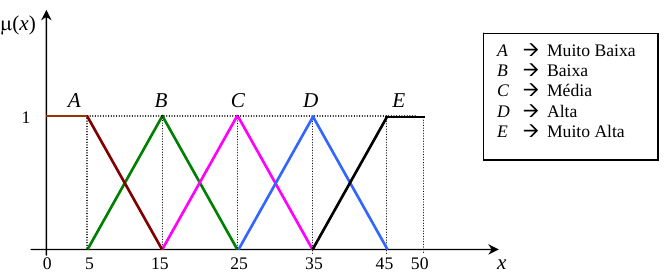
\includegraphics[scale=1]{plot1.png}
\end{figure}


\begin{enumerate}

\item[a)] Encontre as expressões analíticas referentes a cada um dos conjuntos \emph{fuzzy}.

\begin{equation*}
\mu_A (x) = 
\begin{cases} 
1           & \text{se $0 \leq x \leq 5$}
\\
-0,1x+1,5,  & \text{se $5 < x  \leq 15$}
\\
0,          & \text{caso contrário}
\end{cases}
\end{equation*}

\begin{equation*}
\mu_B (x) = 
\begin{cases} 
0,1x-0,5,  & \text{se $5 \leq x  \leq 15$}
\\
-0,1x+2,5,  & \text{se $15 < x  \leq 25$}
\\
0,          & \text{caso contrário}
\end{cases}
\end{equation*}

\begin{equation*}
\mu_C (x) = 
\begin{cases} 
0,1x-1,5,  & \text{se $15 \leq x  \leq 25$}
\\
-0,1x+3,5,  & \text{se $25 < x  \leq 35$}
\\
0,          & \text{caso contrário}
\end{cases}
\end{equation*}

\begin{equation*}
\mu_D (x) = 
\begin{cases} 
0,1x-2,5,  & \text{se $25 \leq x  \leq 35$}
\\
-0,1x+4,5,  & \text{se $35 < x  \leq 45$}
\\
0,          & \text{caso contrário}
\end{cases}
\end{equation*}

\begin{equation*}
\mu_E (x) = 
\begin{cases} 
0,1x-3,5,  & \text{se $35 \leq x  \leq 45$}
\\
1           & \text{se $45 < x \leq 50$}
\\
0,          & \text{caso contrário}
\end{cases}
\end{equation*}

\item[b)] Elabore os procedimentos computacionais que permitam mapear os conjuntos \emph{fuzzy} acima,
utilizando para tanto 1000 pontos de discretização. {Sugestão: Utilize Arrays}. 
\begin{itemize}
\item Para checar o nível de 
generalização do seu sistema, verifique se haverá necessidade de modificações acentuadas quando passarmos 
a trabalhar com 500 ou 2000 pontos de discretização.
\end{itemize}

\item[c)] Elabore os procedimentos computacionais que, dado um valor qualquer de x, permitam
indicar quais dos conjuntos \emph{fuzzy} acima estarão ativos, ou sejam, aqueles que possuem
$\mu(x) \neq 0$.


\item[d)] Elabore os procedimentos computacionais que, dado um conjunto \emph{fuzzy} que está ativo,
retorne o respectivo valor do grau de pertinência em relação a um valor de temperatura x
pertencente ao universo de discurso.


\item[e)] Elabore os procedimentos computacionais que dado um conjunto \emph{fuzzy}, bem como um
valor de grau de pertinência, retorne então o respectivo conjunto crisp representando o $\alpha-
corte$ efetuado.


\end{enumerate}

\item[2] Baseado nos procedimentos computacionais realizados acima faça:
\begin{enumerate}
\item[a)] Imprima numa mesma folha os gráficos (conforme a figura anterior) dos cinco conjuntos
\emph{fuzzy} quando utilizamos 50 e 1000 pontos de discretização para representá-los, explicando
ainda a importância de se especificar corretamente este parâmetro.


\item[b)] Imprima o conjunto \emph{fuzzy} resultante da União dos cinco conjuntos \emph{fuzzy} definidos acima,
utilizando para tanto 1000 pontos de discretização e o operador Máximo.


\item[c)] Imprima o conjunto \emph{fuzzy} resultante da Interseção dos cinco conjuntos \emph{fuzzy} definidos
acima, utilizando para tanto 500 pontos de discretização e o operador Mínimo.


\item[d)] Imprima o conjunto \emph{fuzzy} resultante da operação de Complemento efetuado sobre o
conjunto \emph{fuzzy} C. 
\end{enumerate}



\item[3] Baseado nos procedimentos computacionais realizados no primeiro e segundo exercício,
considerando-se ainda apenas os conjuntos \emph{fuzzy} ativos para uma determinada temperatura,
faça os seguintes gráficos:
\begin{enumerate}
\item[a)] Imprima o conjunto \emph{fuzzy} resultante da União dos conjuntos \emph{fuzzy} ativos em x = 16,75.
\item[b)] Imprima o conjunto \emph{fuzzy} resultante da União dos conjuntos \emph{fuzzy} ativos em x = 37,29.
\item[c)] Imprima o conjunto \emph{fuzzy} resultante da Interseção dos conjuntos \emph{fuzzy} ativos em x = 20.
\item[d)] Imprima o conjunto \emph{fuzzy} resultante da Interseção dos conjuntos \emph{fuzzy} ativos em x = 40.
\end{enumerate}


\item[4] Refaça o exercício anterior adotando os operadores Soma Algébrica (União) e Produto
Algébrico (Interseção).


\item[5] Baseado nos procedimentos computacionais anteriores, imprima então os gráficos resultantes
das seguintes operações:
\begin{enumerate}
\item[a)] $A \cup B \cup C$
\item[b)] $B \cap (C\cup D)$
\item[c)] $(A \cap B) \cup (B \cap C)$
\item[d)] $\overline{A}\cup (B\cap C) \cup \overline{D}$
\end{enumerate}

\end{enumerate}


\newpage

Ex 2a.
\begin{figure}[hptb]
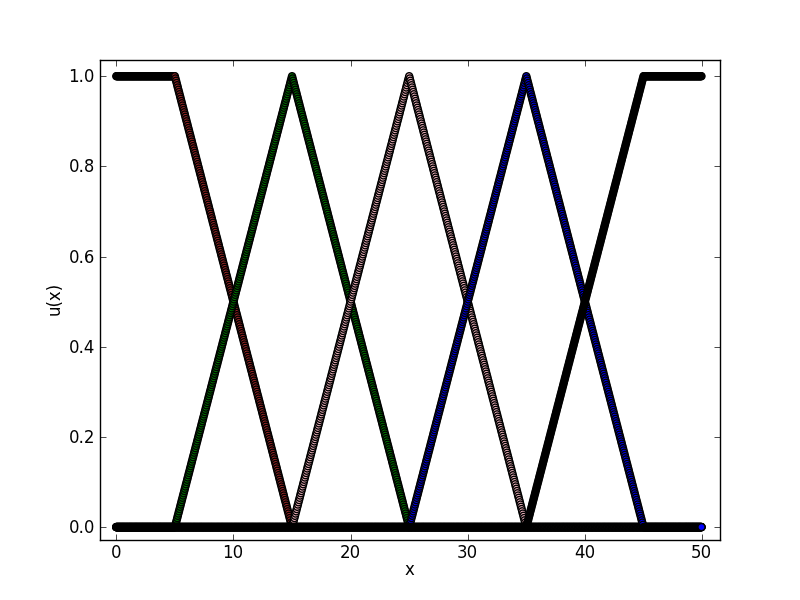
\includegraphics[scale=0.5]{ex1b1000.png}
[]
\end{figure}
\begin{figure}[hptb]
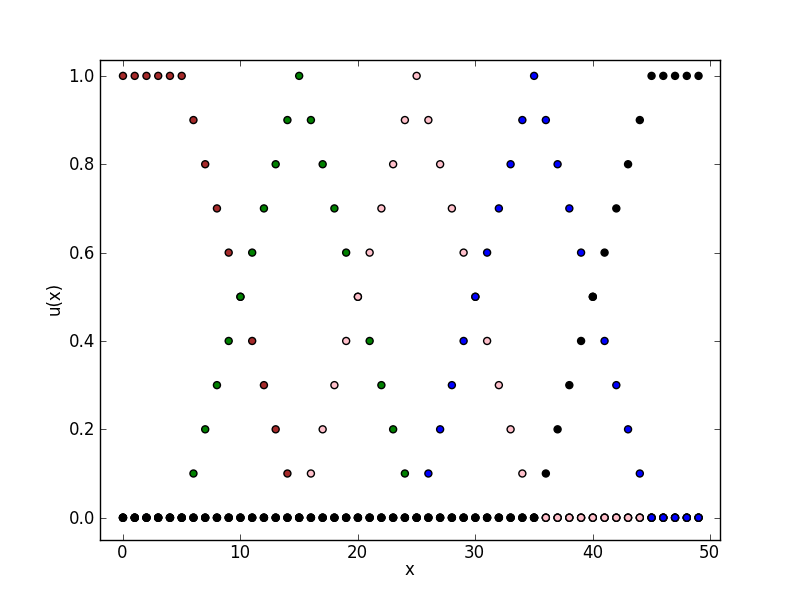
\includegraphics[scale=0.5]{ex2a50.png}
\end{figure}

\newpage
Ex. 2 b, c, d:

\begin{figure}[ht]
        \begin{subfigure}[b]{0.5\textwidth}
                \centering
                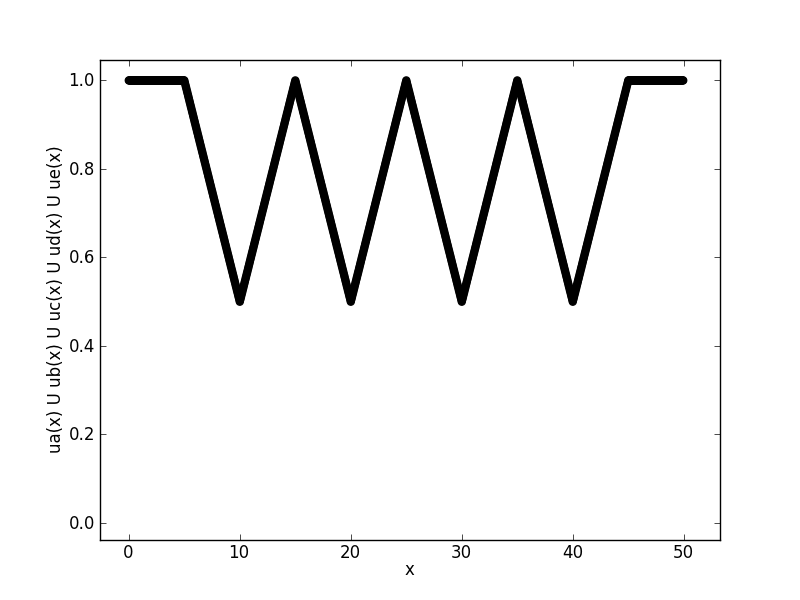
\includegraphics[width=\textwidth]{ex2b.png}
                \caption{2b}
        \end{subfigure}
	\begin{subfigure}[b]{0.5\textwidth}
                \centering
                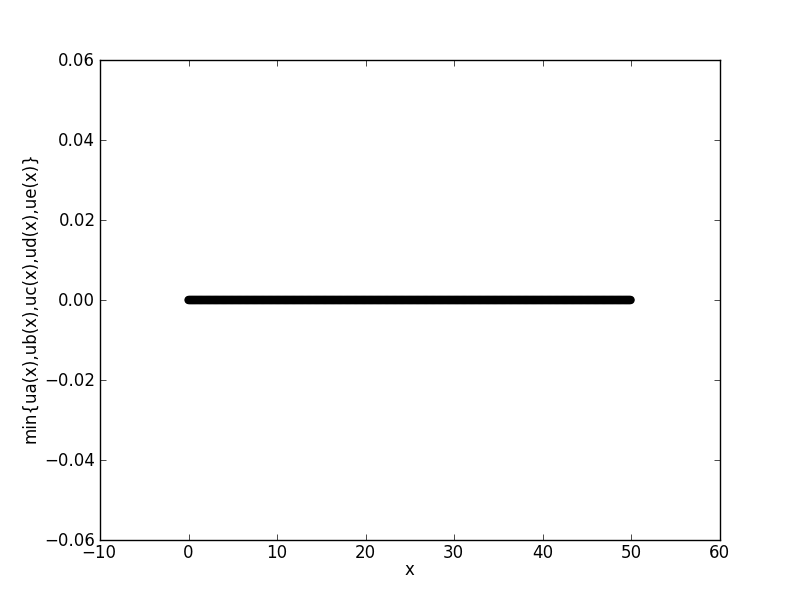
\includegraphics[width=\textwidth]{ex2c.png}
                \caption{2c}
	\end{subfigure}
	\begin{subfigure}[b]{0.5\textwidth}
                \centering
                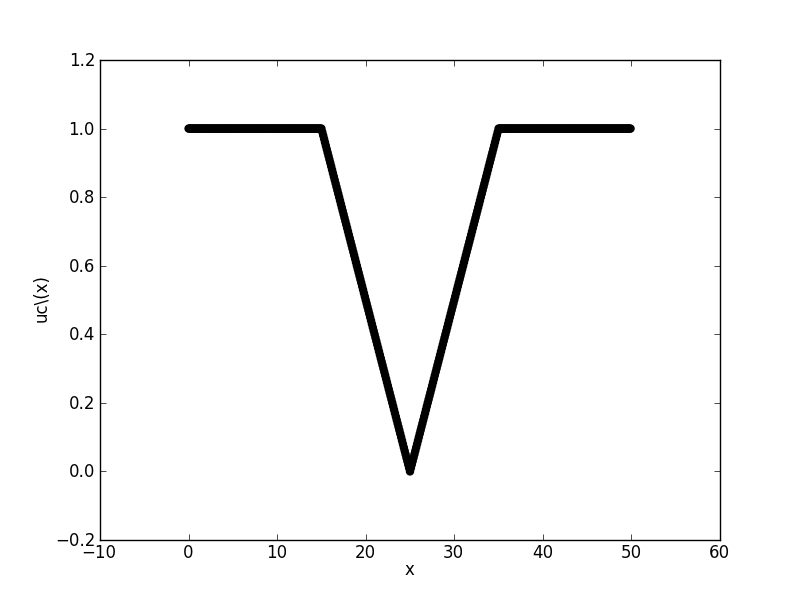
\includegraphics[width=\textwidth]{ex2d.png}
                \caption{2d}
	\end{subfigure}
\end{figure}


\newpage

Ex. 3:
\begin{figure}[ht]
        \begin{subfigure}[b]{0.5\textwidth}
                \centering
                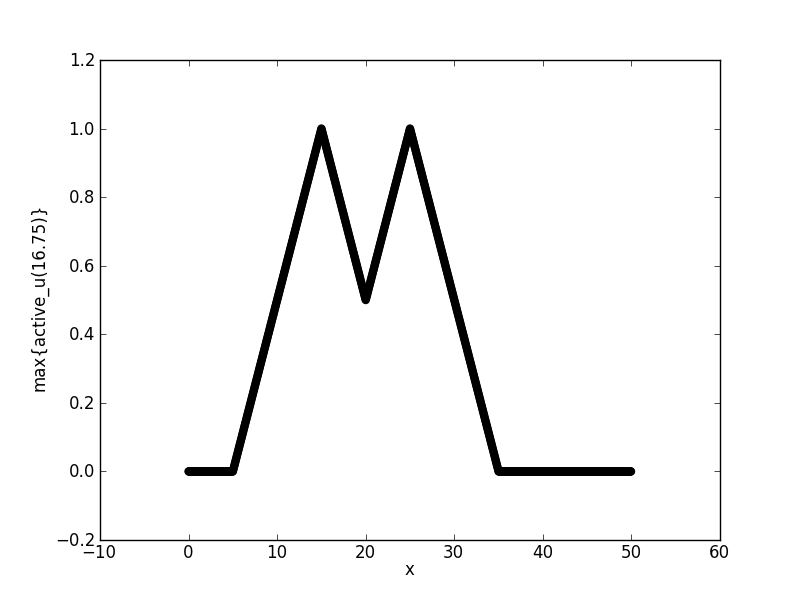
\includegraphics[width=\textwidth]{ex3a.png}
                \caption{3a}
        \end{subfigure}
	\begin{subfigure}[b]{0.5\textwidth}
                \centering
                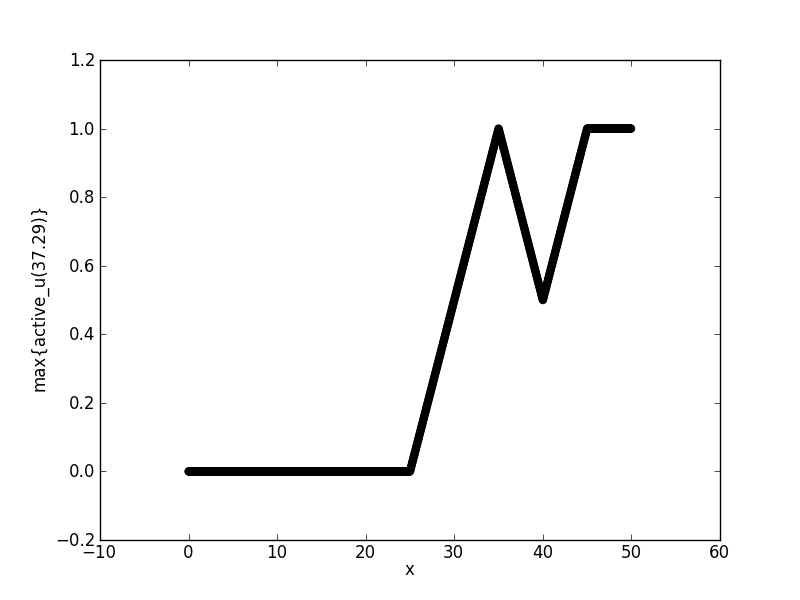
\includegraphics[width=\textwidth]{ex3b.png}
                \caption{3b}
	\end{subfigure}
	\begin{subfigure}[b]{0.5\textwidth}
                \centering
                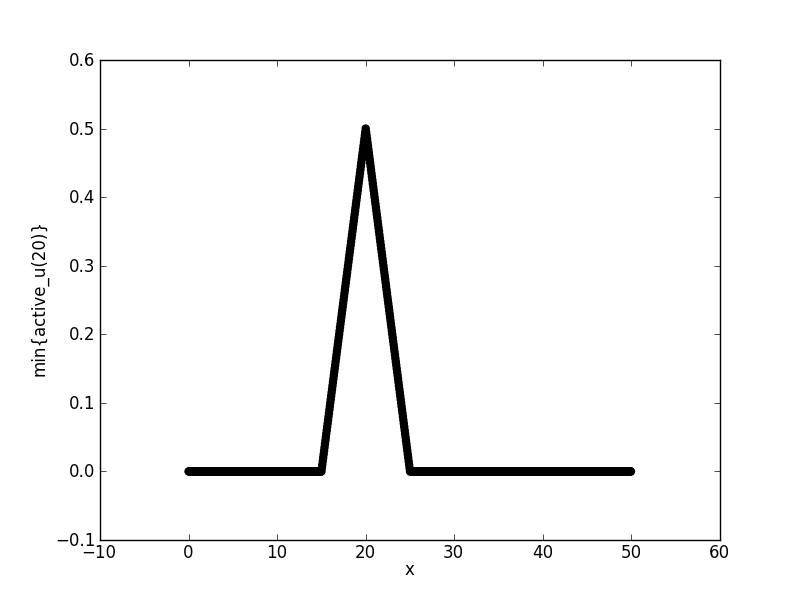
\includegraphics[width=\textwidth]{ex3c.png}
                \caption{3c}
	\end{subfigure}
	\begin{subfigure}[b]{0.5\textwidth}
                \centering
                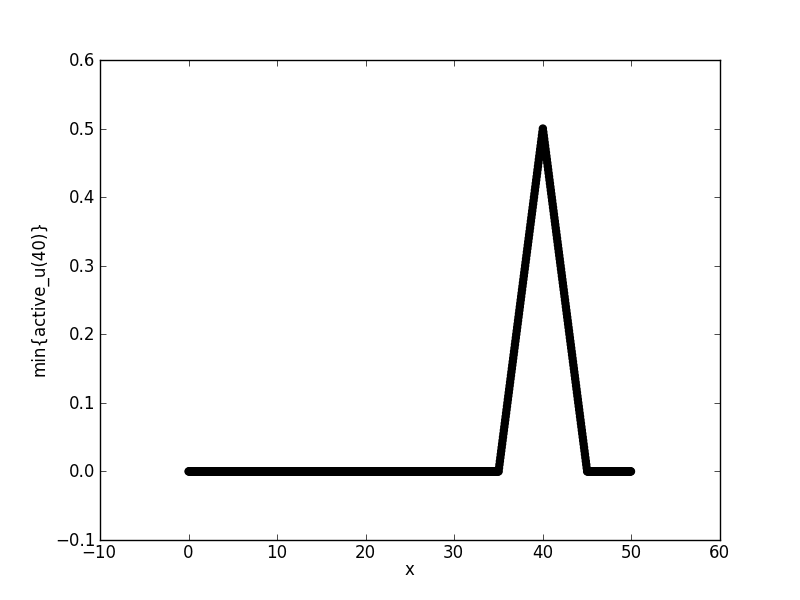
\includegraphics[width=\textwidth]{ex3d.png}
                \caption{3d}
	\end{subfigure}
\end{figure}


\newpage

Ex. 4:
\begin{figure}[ht]
        \begin{subfigure}[b]{0.5\textwidth}
                \centering
                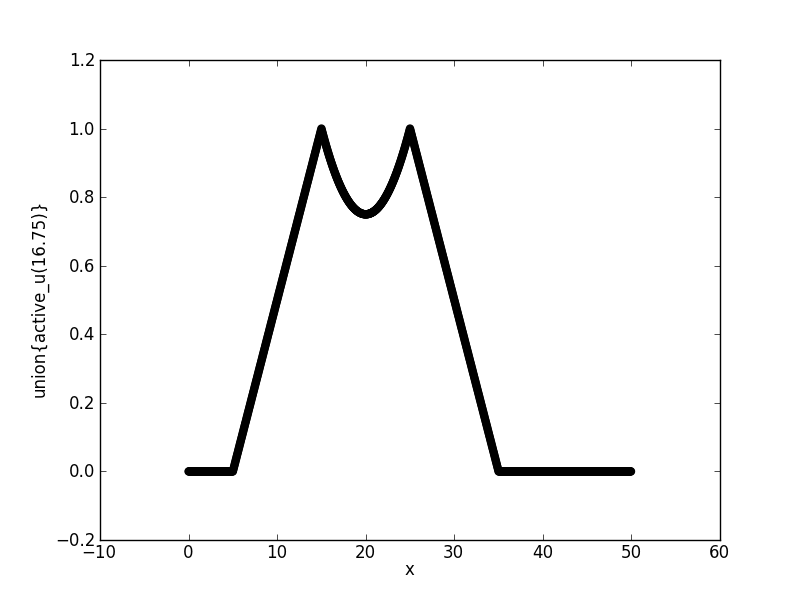
\includegraphics[width=\textwidth]{ex4a.png}
                \caption{4a}
        \end{subfigure}
	\begin{subfigure}[b]{0.5\textwidth}
                \centering
                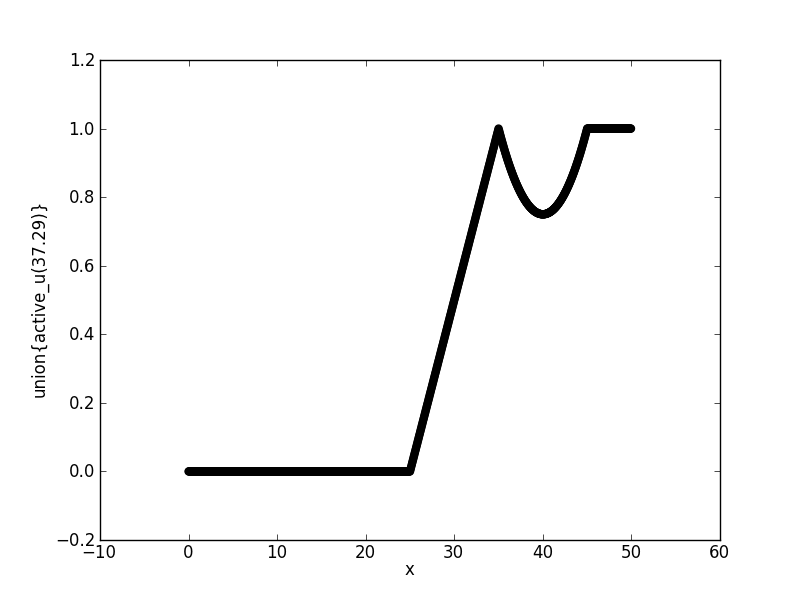
\includegraphics[width=\textwidth]{ex4b.png}
                \caption{4b}
	\end{subfigure}
	\begin{subfigure}[b]{0.5\textwidth}
                \centering
                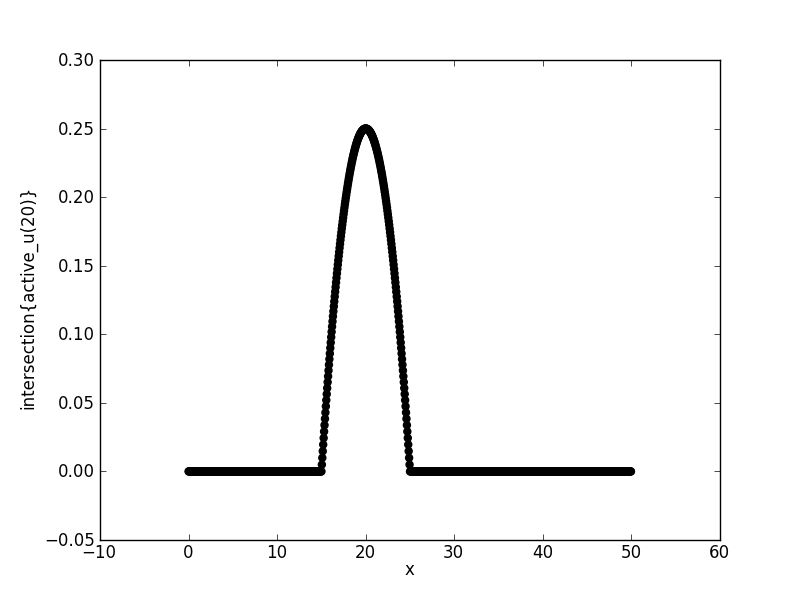
\includegraphics[width=\textwidth]{ex4c.png}
                \caption{4c}
	\end{subfigure}
	\begin{subfigure}[b]{0.5\textwidth}
                \centering
                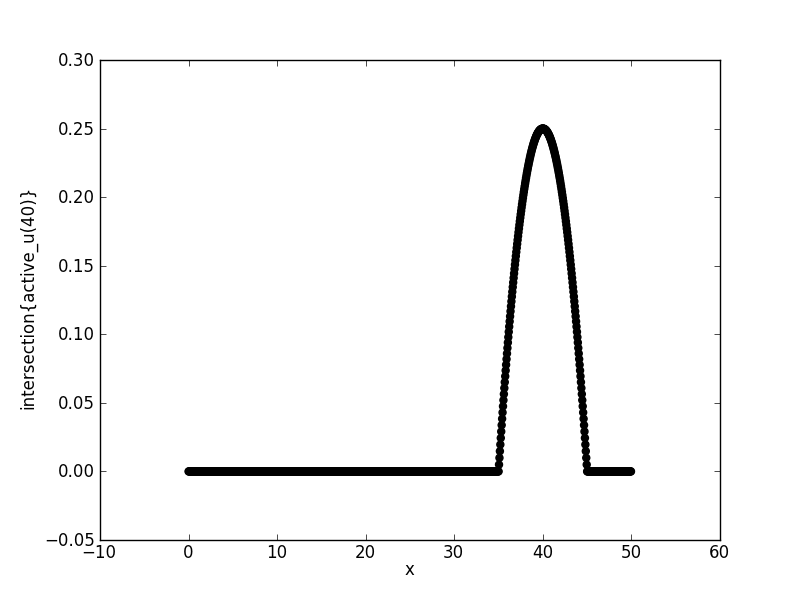
\includegraphics[width=\textwidth]{ex4d.png}
                \caption{4d}
	\end{subfigure}
\end{figure}


\newpage
Ex. 5:
\begin{figure}[ht]
        \begin{subfigure}[b]{0.5\textwidth}
                \centering
                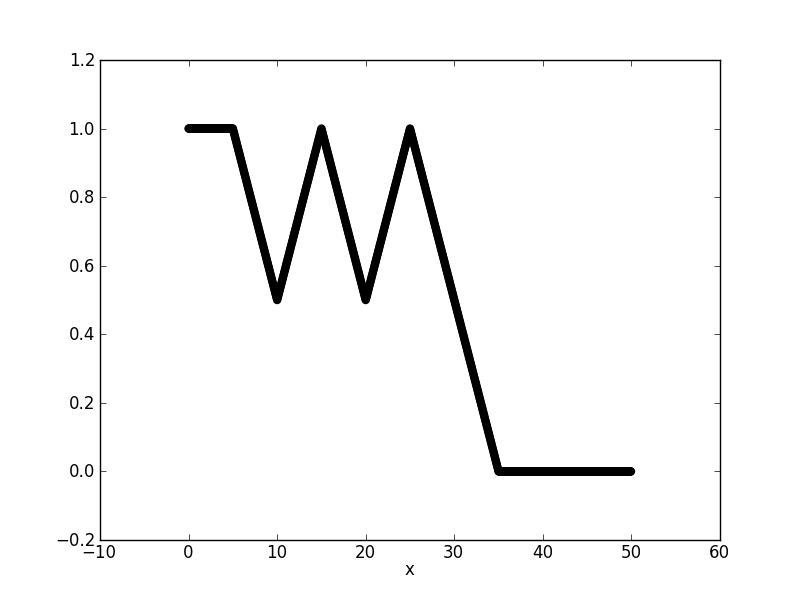
\includegraphics[width=\textwidth]{ex5a.png}
                \caption{5a}
        \end{subfigure}
	\begin{subfigure}[b]{0.5\textwidth}
                \centering
                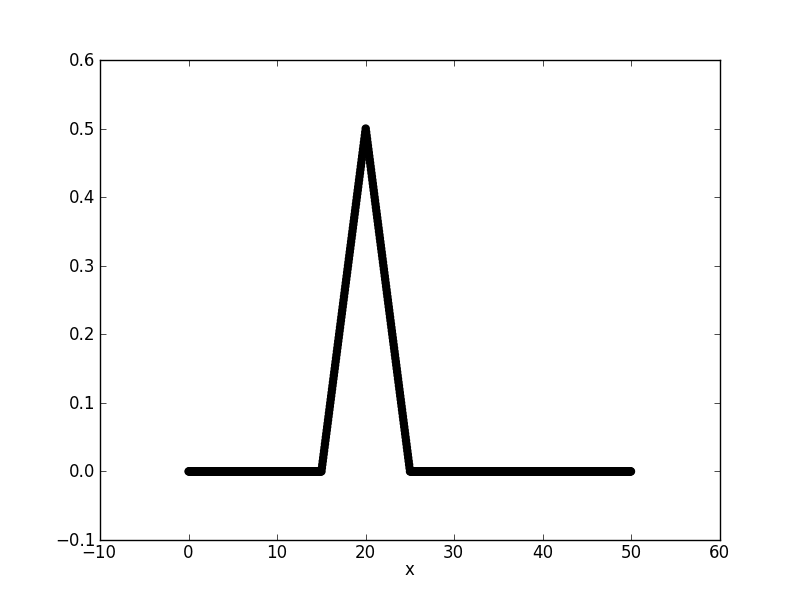
\includegraphics[width=\textwidth]{ex5b.png}
                \caption{5b}
	\end{subfigure}
	\begin{subfigure}[b]{0.5\textwidth}
                \centering
                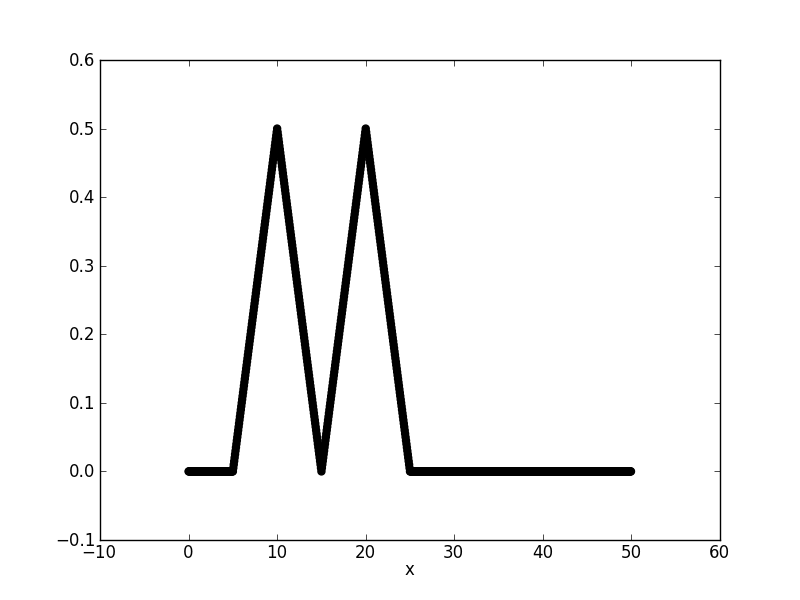
\includegraphics[width=\textwidth]{ex5c.png}
                \caption{5c}
	\end{subfigure}
	\begin{subfigure}[b]{0.5\textwidth}
                \centering
                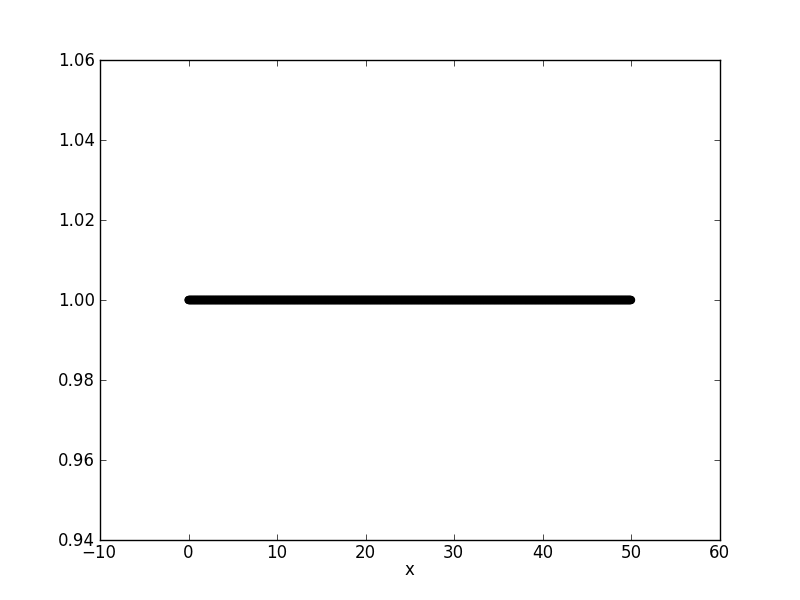
\includegraphics[width=\textwidth]{ex5d.png}
                \caption{5d}
	\end{subfigure}
\end{figure}


\newpage
\lstinputlisting[language=Python]{ex1.py}

\end{document}
